\documentclass[]{article}
\usepackage{lmodern}
\usepackage{amssymb,amsmath}
\usepackage{ifxetex,ifluatex}
\usepackage{fixltx2e} % provides \textsubscript
\ifnum 0\ifxetex 1\fi\ifluatex 1\fi=0 % if pdftex
  \usepackage[T1]{fontenc}
  \usepackage[utf8]{inputenc}
\else % if luatex or xelatex
  \ifxetex
    \usepackage{mathspec}
  \else
    \usepackage{fontspec}
  \fi
  \defaultfontfeatures{Ligatures=TeX,Scale=MatchLowercase}
\fi
% use upquote if available, for straight quotes in verbatim environments
\IfFileExists{upquote.sty}{\usepackage{upquote}}{}
% use microtype if available
\IfFileExists{microtype.sty}{%
\usepackage[]{microtype}
\UseMicrotypeSet[protrusion]{basicmath} % disable protrusion for tt fonts
}{}
\PassOptionsToPackage{hyphens}{url} % url is loaded by hyperref
\usepackage[unicode=true]{hyperref}
\hypersetup{
            pdftitle={t-test Power Simulation},
            pdfauthor={Kyle Dettloff},
            pdfborder={0 0 0},
            breaklinks=true}
\urlstyle{same}  % don't use monospace font for urls
\usepackage[margin=0.5in]{geometry}
\usepackage{longtable,booktabs}
% Fix footnotes in tables (requires footnote package)
\IfFileExists{footnote.sty}{\usepackage{footnote}\makesavenoteenv{long table}}{}
\usepackage{graphicx,grffile}
\makeatletter
\def\maxwidth{\ifdim\Gin@nat@width>\linewidth\linewidth\else\Gin@nat@width\fi}
\def\maxheight{\ifdim\Gin@nat@height>\textheight\textheight\else\Gin@nat@height\fi}
\makeatother
% Scale images if necessary, so that they will not overflow the page
% margins by default, and it is still possible to overwrite the defaults
% using explicit options in \includegraphics[width, height, ...]{}
\setkeys{Gin}{width=\maxwidth,height=\maxheight,keepaspectratio}
\IfFileExists{parskip.sty}{%
\usepackage{parskip}
}{% else
\setlength{\parindent}{0pt}
\setlength{\parskip}{6pt plus 2pt minus 1pt}
}
\setlength{\emergencystretch}{3em}  % prevent overfull lines
\providecommand{\tightlist}{%
  \setlength{\itemsep}{0pt}\setlength{\parskip}{0pt}}
\setcounter{secnumdepth}{0}
% Redefines (sub)paragraphs to behave more like sections
\ifx\paragraph\undefined\else
\let\oldparagraph\paragraph
\renewcommand{\paragraph}[1]{\oldparagraph{#1}\mbox{}}
\fi
\ifx\subparagraph\undefined\else
\let\oldsubparagraph\subparagraph
\renewcommand{\subparagraph}[1]{\oldsubparagraph{#1}\mbox{}}
\fi

% set default figure placement to htbp
\makeatletter
\def\fps@figure{htbp}
\makeatother

\let\rmarkdownfootnote\footnote%
\def\footnote{\protect\rmarkdownfootnote}
\usepackage{titling}
\setlength{\droptitle}{-2em}
\pretitle{\vspace{\droptitle}\centering\huge}
\posttitle{\par}
\preauthor{\centering\large\emph}
\postauthor{\par}
\predate{\centering\large\emph}
\postdate{\par}

\title{t-test Power Simulation}
\author{Kyle Dettloff}
\date{04-09-2020}

\begin{document}
\maketitle

\pagenumbering{gobble}

\textbf{Simulation 1:} n\textsubscript{1} = 10, n\textsubscript{2} = 10,
sd\textsubscript{1} = 1, sd\textsubscript{2} = 1, unequal variance\\
\textbf{Simulation 2:} n\textsubscript{1} = 10, n\textsubscript{2} = 20,
sd\textsubscript{1} = 1, sd\textsubscript{2} = 3, unequal variance\\

\begin{center}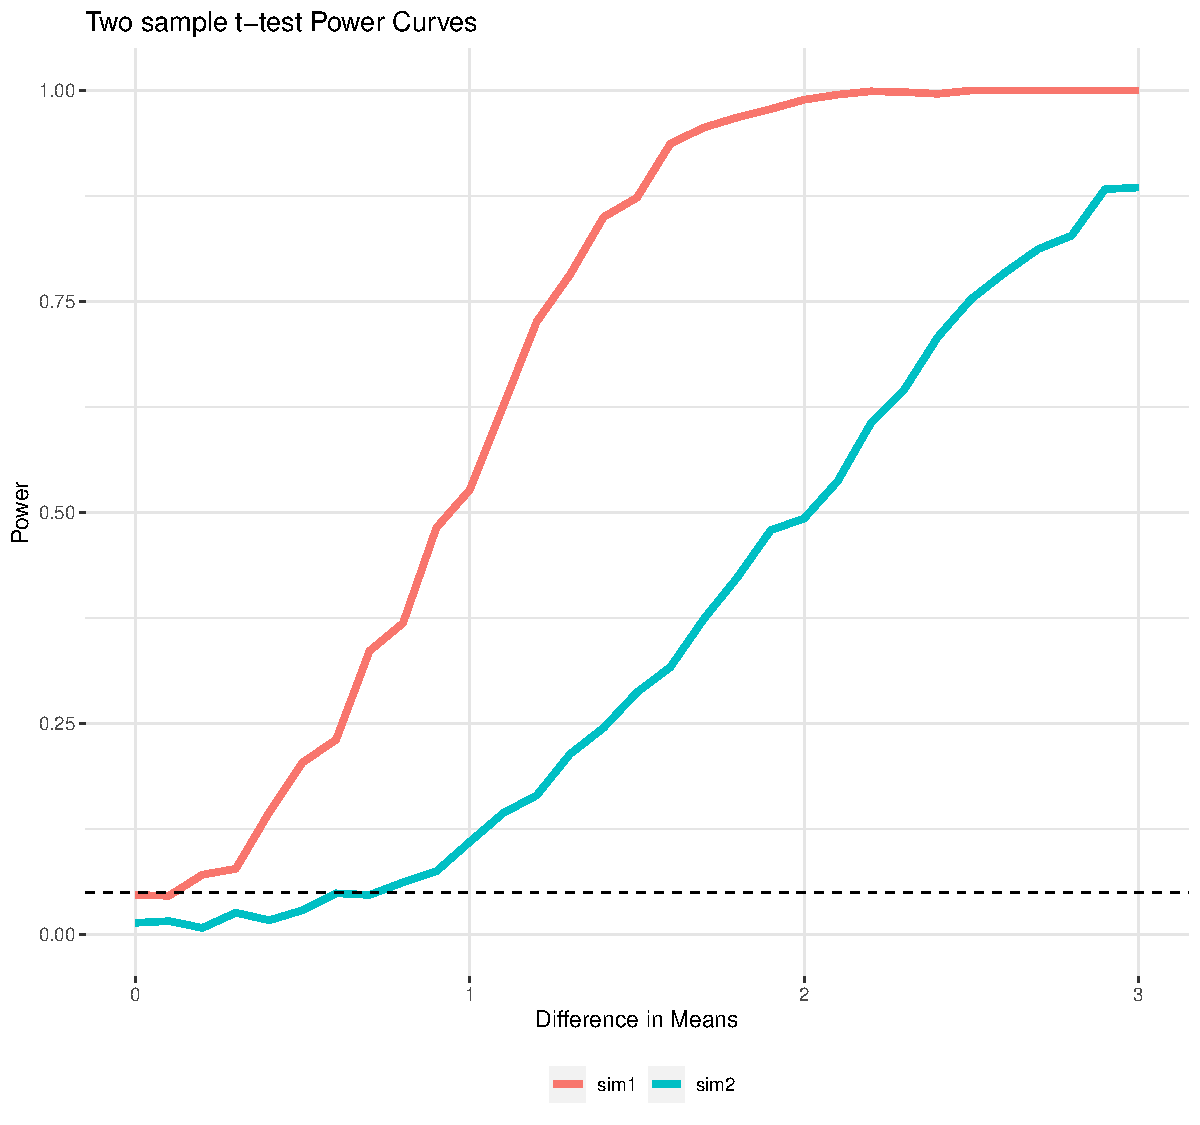
\includegraphics{markdownExample_files/figure-latex/unnamed-chunk-2-1} \end{center}

\newpage

\begin{longtable}[]{@{}rrr@{}}
\caption{H\textsubscript{0} Rejection Rates, alpha =
0.05}\tabularnewline
\toprule
Difference in Means & Simulation 1 & Simulation 2\tabularnewline
\midrule
\endfirsthead
\toprule
Difference in Means & Simulation 1 & Simulation 2\tabularnewline
\midrule
\endhead
0.0 & 0.047 & 0.014\tabularnewline
0.1 & 0.046 & 0.016\tabularnewline
0.2 & 0.071 & 0.008\tabularnewline
0.3 & 0.078 & 0.026\tabularnewline
0.4 & 0.145 & 0.017\tabularnewline
0.5 & 0.204 & 0.029\tabularnewline
0.6 & 0.231 & 0.049\tabularnewline
0.7 & 0.336 & 0.047\tabularnewline
0.8 & 0.369 & 0.062\tabularnewline
0.9 & 0.482 & 0.075\tabularnewline
1.0 & 0.527 & 0.110\tabularnewline
1.1 & 0.626 & 0.144\tabularnewline
1.2 & 0.726 & 0.165\tabularnewline
1.3 & 0.782 & 0.214\tabularnewline
1.4 & 0.850 & 0.245\tabularnewline
1.5 & 0.873 & 0.287\tabularnewline
1.6 & 0.937 & 0.317\tabularnewline
1.7 & 0.956 & 0.374\tabularnewline
1.8 & 0.968 & 0.423\tabularnewline
1.9 & 0.978 & 0.479\tabularnewline
2.0 & 0.989 & 0.493\tabularnewline
2.1 & 0.995 & 0.537\tabularnewline
2.2 & 0.999 & 0.606\tabularnewline
2.3 & 0.998 & 0.646\tabularnewline
2.4 & 0.996 & 0.708\tabularnewline
2.5 & 1.000 & 0.753\tabularnewline
2.6 & 1.000 & 0.784\tabularnewline
2.7 & 1.000 & 0.812\tabularnewline
2.8 & 1.000 & 0.828\tabularnewline
2.9 & 1.000 & 0.883\tabularnewline
3.0 & 1.000 & 0.885\tabularnewline
\bottomrule
\end{longtable}

\end{document}
